\chapter{Approximate Inference for Stochastic Epidemic Models of Outbreaks in Large Populations}
\label{chap:lna_for_sems}

\section{Overview}
\label{sec:lna_overview}

Surveillance and outbreak response systems often report incidence counts of new cases detected in each inter--observation time interval. Analyzing this type of time series data is challenging since we must overcome many of the same challenges that we face in modeling the transmission dynamics of infectious diseases in small population settings with prevalence data --- discrete snapshots of a continuously evolving epidemic process, detecting a fraction of the new cases, and often directly observing only one aspect of the disease process. Furthermore, our task is made more difficult by the additional computational burden that results from repeated evaluation of CTMC likelihoods; the products of exponential waiting time distributions consist of polynomially increasing numbers of terms, and agent--based data augmentation (DA) MCMC algorithms become unwieldy as the numbers of subject--path proposals required to meaningfully perturb the CTMC likelihood get large \citep{fintzi2017efficient}. 

In this chapter, we show how the LNA of Section \ref{subsubsec:lna_background} can be adapted to obtain approximate inference for SEMs fit to epidemic count data in large populations. Our contributions are threefold: First, we demonstrate how the SEM dynamics should be reparameterized so that the LNA can be used to approximate transition densities of the counting processes for disease state transition events. Second, we fold the LNA into a Bayesian DA framework in which latent LNA paths are sampled using the elliptical slice sampling (EliptSS) algorithm of \cite{murray2010}. This provides us with general machinery for jointly updating the latent paths while absolving us of the \textit{de facto} modeling choice that the data be Gaussian in order to efficiently perform inference as in \cite{fearnhead2014,komorowski2009}, or the need to use computationally intensive particle filter methods for non--Gaussian emission distributions as in \cite{golightly2015delayed}. Finally, we introduce a non--centered parameterization for the LNA that massively improves the efficiency of our DA MCMC framework and makes it tractable for fitting complex models. 

\section{Fitting Stochastic Epidemic Models via the Linear Noise Approximation}
\label{sec:lna_methods}

For clarity, we will present the algorithm for fitting SEMs via the LNA in the context of fitting the susceptible--infected--recovered (SIR) model to Poisson distributed incidence counts. We will, however, provide notation where appropriate so that the generality of the algorithm should be apparent. The SIR model is an abstraction of the transmission dynamics of an outbreak as a closed, homogeneously mixing population of $ N $ exchangeable individuals who are either susceptible $ (S) $, infected, and hence infectious, $ (I) $, or recovered $ (R) $. It is important to note that the model compartments refer to disease states as they relate to the transmission dynamics, not the disease process. Thus, an individual is considered to be recovered when she no longer has infectious contact with other individuals in the population, not when she clears disease carriage. As another example, in the susceptible--exposed--infected--recovered (SEIR) type models that we will consider later, the latent period in which an individual is exposed, but not yet infectious, should be understood as possibly varying in population with different contact dynamics, even when the incubation period of the pathogen should arguably be consistent across groups.

\subsection{Measurement Process and Data}
\label{subsec:lna_measproc}
Incidence data, $ \bY = \lbrace Y_1,\dots,Y_L\rbrace $,  arise as increments of the numbers of new cases accumulated in a set of time intervals, $ \mcI = \lbrace\mcI_1,\dots,\mcI_L:\ \mcI_\ell = (t_{\ell-1},t_\ell]\rbrace $. In outbreak or surveillance settings, we do not typically believe that every case is detected since individuals may be asymptomatic or may escape detection. Let $ \bN^c = (N^c_{SI}, N^c_{IR}) $ denote the counting process for the cumulative numbers of infections ($ S\rightarrow I $ transitions) and recoveries ($ I\rightarrow R $ transitions), and let $ \Delta \bN^c(t_\ell) = \bN^c(t_\ell) - \bN^c(t_{\ell-1})$ denote the change in cumulative numbers of transitions over $ \mcI_\ell $; so, $ \Delta N^c_{SI}(t_\ell)$ is the incidence over $ (t_{\ell-1},t_\ell] $. We might choose to model the number of observed cases as a Poisson sample of the true incidence with detection rate $ \rho $. Thus,
\begin{equation}
\label{eqn:incidence_emitprob}
Y_\ell|\Delta N^c_{SI}(t_\ell),\rho \sim \mr{Pois}(\rho\Delta N^c_{SI}(t_\ell)).
\end{equation}

There are two minor points that we wish to make note of before proceeding. First, we have allowed for the possibility that cases are over--reported. This is neither a necessary assumption for any of the subsequent results, nor is it unreasonable when studying outbreaks in large populations where the ``fog of war" might lead to inflation of reported incidence or misclassification of individuals whose symptoms are similar to the disease of interest. This modeling choice is also not particularly problematic when the detection probability is low since the emission densities will have negligible mass above the true incidence. Second, we are also making this modeling choice with an eye on the compatibility of the measurement distribution with the eventual LNA approximation, which takes real, not integer, values. The Poisson distribution, along with the negative binomial distribution that we will use in subsequent sections, are well defined for non--integer values of the mean parameter. 

\subsection{Latent Epidemic Process}
\label{subsec:lna_epid_proc}

The SIR model is typically expressed in terms of compartment counts, $ \bX^c = \lbrace S^c,I^c,R^c\rbrace $, that evolve in continuous time on state space $ \mcS_X^c = \left \lbrace \mcC_{lmn}:l,m,n\in\lbrace0,\dots,N\rbrace,\ l+m+n=P\right \rbrace $. We will make the (not particularly limiting) modeling choice to express the waiting times between disease state transitions as being exponentially distributed. Thus, $ \bX $ evolves according to a Markov jump process (MJP). If our data had consisted of prevalence counts, which arise as partial observations of infected individuals, we might have chosen to approximate transition densities of the MJP for $ \bX $ in the usual way that appears in \cite{komorowski2009,fearnhead2014}. 

However, incidence data are discretely observed, partial realizations of the increments of counting processes that evolve continuously in time as individuals transition among disease states. The emission probabilities for incidence data, e.g., (\ref{eqn:incidence_emitprob}), depend on the change in $ N_{SI}^c $ over the time interval $ (t_{\ell-1},t_\ell] $, not on the change in $ I $ over the interval. It would be incorrect to treat incidence as simply the difference in prevalence. We could easily construct a scenario where there are positive numbers of infections, but where the prevalence does not change due to an equal number of recoveries. We need to construct the LNA that approximates transition densities of $ \bN $ if we are to write down correctly specified emission probabilities.

The cumulative incidence process for infections and recoveries, $ \bN^c $, is a Markov jump process state space $ \mcS_N^c = \left \lbrace \mcC_{jk}:j,k\in\lbrace0,\dots,N\rbrace\right \rbrace $. Let $ \beta $ denote the per--contact infection rate, and $ \mu $ denote the rate at which each infected individual recovers. The rate at which $ \bN^c $ transitions from state $ \bn $ to $ \bn^{\prime}$ is 
\begin{equation}
	\label{eqn:lna_sir_rates}
	\blambda_{\bn,\bn^\prime} = \left \lbrace \begin{array}{ll}
	\lambda_{SI} = \beta S I, & \bn = (n_{SI},n_{IR}),\ \bn^\prime = (n_{SI}+1,n_{IR}),\text{ and } n_{SI}+1\leq P, \\
	 \lambda_{IR} = \mu I, &  \bn = (n_{SI},n_{IR}),\  \bn^\prime = (n_{SI},n_{IR}+1),\text{ and } n_{IR}+1\leq P, \\
	 0, & \text{for all other } \bn \text{ and } \bn^\prime.
	\end{array} \right.
\end{equation}

\subsection{Tractable Approximations for Intractable Likelihoods}
\label{subsec:lna_motivation}
We would like to make inferences about the posterior distribution of the parameters, e.g., $ \btheta = (\beta, \mu, \bX(t_0), \rho)$, that govern the latent epidemic process and sampling distribution, 
\begin{align}
\label{eqn:intractable_posterior}
 \pi(\btheta|\bY)&\propto \pi(\bY|\btheta)\pi(\btheta) = \int L(\bY|\bN^c,\btheta)\pi(\bN^c|\btheta)\pi(\btheta)\rmd\pi(\bN^c)\nonumber\\
 &= \int_{\mcS^c}\prod_{\ell=1}^L \Pr\left (\bY_\ell|\Delta\bN_{SI}^c(t_\ell),\btheta\right )\pi\left (\bN^c(t_\ell)|\bn^c(t_{\ell-1}),\btheta\right )\pi(\btheta)\rmd\pi(\bN^c)
\end{align}
where $ \pi(\btheta) $ specifies the prior density of the model parameters. However, this integral is analytically intractable and is challenging to compute numerically due to the size of the state space of $ \bN^c $. In the following subsections, we will obtain the LNA for transition densities of $ \bN^c $, turning (\ref{eqn:intractable_posterior}) into an integral over a much more computationally tractable product of Gaussian densities and non--Gaussian emission probabilities. As we shall see, approximating the complete data likelihood in the posterior $ \pi(\btheta,\bN^c|\btheta) $ with a Gaussian state space model will open the doors to efficient algorithms for sampling from the approximate posterior. 

\subsection{Diffusion Approximation}
\label{subsec:diff_approx}

As outlined in Section \ref{subsubsec:diff_approx}, there are a variety of methods for arriving at a diffusion approximation for a Markov jump process, which under certain conditions yield equivalent results (for a comprehensive reference, see \cite{fuchs2013inference}). In the interest of clarity, we follow \cite{fearnhead2014,golightly2013simulation,golightly2015delayed,wilkinson2011stochastic} and appeal to an intuitive, though somewhat informal, construction of the CLE by matching its drift and diffusion with the approximate moments of increments of the MJP path in infinitesimal time intervals. For more detailed presentations see \cite{fuchs2013inference,gillespie2000chemical,wallace2012linear}. 

Suppose that, at the current time, the compartment counts are given by $ \bX^c(t) = \bx^c_t $. We are interested in approximating the numbers of infections and recoveries in a small time interval, $ (t, t+\dt] $, i.e., $ \bN^c(t+\dt) - \bN(t)$. Now, suppose that we can choose $ \dt $ such that the following two \textit{leap} conditions hold:

\begin{enumerate}
	\item $ \dt $ is sufficiently \textit{small} that the $ \bX^c $ is essentially unchanged over $ (t,t+\dt] $, so that the rates of infections and recoveries are approximately constant: 
	\begin{equation}\label{eqn:tau_cond_1}
	\blambda(\bX^c(t^\prime)) \approx \blambda(\bx^c(t)),\ \forall t^\prime \in (t,t+\dt].
	\end{equation}
	\item $ \dt $ is sufficiently \textit{large} that we can expect many disease state transitions of each type:
	\begin{equation}\label{eqn:tau_cond_2}
	\blambda(\bx^c(t)) \gg \bs{1}.
	\end{equation}
\end{enumerate}

Condition (\ref{eqn:tau_cond_1}), which can be trivially satisfied just by choosing $ \dt $ to be small, implies that the numbers of infections and recoveries in $ (t,t+\dt] $ are essentially independent of one another since the rates at which they occur are approximately constant within the interval \cite{gillespie2000chemical}. This condition also carries the stronger implication that the numbers of infections and recoveries in the interval are independent Poisson random variables with rates $ \blambda(\bx^c(t)\dt) $, i.e., $ N^c_{SI}(\dt) \sim \mr{Poisson}(\beta S(t)I(t)\dt) $ and $ N^c_{IR}(t+\dt) \sim \mr{Poisson}(\mu I(t)\dt) $. Condition (\ref{eqn:tau_cond_2}), which we can reasonably expect to be satisfied in large populations where transmission dynamics are near their deterministic ODE limits \cite{wallace2012linear}, implies that the Poisson distributed increments can be well approximated by independent Gaussian random variables. 

Thus, (\ref{eqn:tau_cond_1}) and (\ref{eqn:tau_cond_2}) are satisfied, we can approximate the integer--valued processes, $ \bX^c $ and $ \bN^c $, with the real--valued processes, $ \bX $ and $ \bN $. For the SIR model, the state space of $ \bX $ is $ \mcS_X^R = \lbrace \mcV_{lmn}:l,m,n \in [0,N],\ l+m+n=P\rbrace $, and the state space  of $ \bN $ is $ \mcS_N^R = \lbrace \mcV_{jk}: j,k \in [0,N] \rbrace $. More generally, the state space of $ \bX $ will be the set of compartment volumes that are non--negative and that sum to the population size, while the state space of $ \bN $ is the set of non--decreasing and non--negative incidence paths, constrained so that they do not lead to invalid prevalence paths (e.g., if at some point there are more recoveries than infections, which would lead to a negative number of infected individuals). For now, we will ignore the constraints on $ \mcS_N^R $ and $ \mcS_X^R $, and approximate the changes in cumulative incidence of infections and recoveries in an infinitesimal time step as 
\begin{equation}
\bN(t+\dt) - \bN(t) \approx \blambda(\bX(t))\dt + \bLambda(\bX(t))^{1/2}\dt^{1/2}\bZ,
\end{equation}
where $ \bLambda = \diag\left (\blambda(\bX) \right )$ and $ \bZ\sim MVN(\bs{0},\mb{I}) $. This implies the equivalent CLE,
\begin{equation}
\label{eqn:sir_cle_X}
\rmd \bN(t) = \blambda(\bX(t))\dt + \bLambda(\bX(t))^{1/2}\rmd\bW_t, 
\end{equation}
where $ \bW_t $ is a vector of independent Brownian motion and $ \bLambda(\bX(t))^{1/2} $ denotes the matrix square root of $ \bLambda(\bX(t)) $. 

\subsubsection{Reparameterizating the CLE in terms of incidence}
\label{subsubsec:cle_repar}
The LNA of (\ref{eqn:sir_cle_X}) will involve derivatives of the rates, $ \blambda $, with respect to the incidence process, $ \bN $. In order to enable us to compute these derivatives, we borrow from \cite{breto2009time,ho2016direct} a reparameterization for $ \bX (t)$ in terms of $ \bN(t) $, conditional on the initial conditions $ \bX(t) = \bx_0 $ and $ \bN(t) = \bs{0} $. Let $ \bA $ denote the matrix whose rows specify changes in counts of susceptible, infected, and recovered individuals corresponding to one infection or recovery event:
\begin{equation}
\label{eqn:sir_stoich}
\bA = \kbordermatrix{& S & I &  R\\
	S\rightarrow I& -1& 1 & 0\\
	I \rightarrow R & 0& -1 & 1
}.
\end{equation}

Now, $ \bX $ is coupled to $ \bN $ via the relationship,
\begin{equation}
\label{eqn:incid2prev}
\bX(t) = \bx_0 + \bA^T\bN(t).
\end{equation}
For the SIR model, 
\begin{align}
\left (\begin{array}{c}
S(t) \\
I(t) \\
R(t)
\end{array}\right ) &= \left (\begin{array}{c}
S_0 - N_{SI}(t) \\
I_0 + N_{SI}(t) - N_{IR}(t) \\
R_0 + N_{IR}(t)
\end{array}\right ),
\end{align}
which enables us to rewrite (\ref{eqn:sir_cle_X}) as
\begin{align}
\label{eqn:sir_cle_N}
 \rmd\bN(t)&= \blambda(\bN(t))\dt + \bLambda(\bN(t))^{1/2}\rmd\bW_t \\
 &= \left (\begin{array}{cc}
\beta (S_0 - N_{SI}(t))(I_0 + N_{SI}(t) - N_{IR}(t))\\
\mu(I_0 + N_{IR}(t))\dt 
\end{array}\right )\dt + \nonumber\\
&\hspace{0.5in}\left(\begin{array}{cc}
\beta (S_0 - N_{SI}(t))(I_0 + N_{SI}(t) - N_{IR}(t)) & 0 \\
0 & \mu(I_0 + N_{IR}(t))
\end{array}\right)^{1/2}\rmd\bW_t. \nonumber 
\end{align}

\subsubsection{Log transforming the CLE}
\label{subsubsec:log_cle}
Changes in compartment volumes affect the rates, and hence increments in the incidence process, multiplicatively. Therefore, from a scientific perspective, we would like for perturbations about the drift in (\ref{eqn:sir_cle_N}) to be symmetric on a multiplicative, not an additive scale. Hence, we log transform (\ref{eqn:sir_cle_N}). Let $ \bNtil = \log(\bN + \bs{1}) \implies\bN = \exp(\bNtil) - \bs{1}$. By It\^{o}'s lemma \cite{oksendal2003stochastic}, the corresponding SDE for $ \bNtil $ is 
	\begin{align}
\label{eqn:sir_log_cle}
\rmd\bNtil(t) &= \diag\left (\exp(-\bNtil(t)) - 0.5\exp(-2\bNtil(t))\right )\blambda\left (\exp(\bNtil(t))-\bs{1}\right )\dt\ + \nonumber\\
& \hspace{0.5in} \diag\left (\exp(-\bNtil(t))\right )\bLambda\left (\exp(\bNtil(t))-1\right )^{1/2}\rmd\bW_t \\
\label{eqn:sir_log_cle_gen}
&= \boeta(\bNtil(t))\dt + \bPhi(\bNtil(t))^{1/2}\rmd\bW_t
\end{align}

\subsection{Linear Noise Approximation}
\label{subsec:sir_lna}

In Section \ref{subsubsec:lna_background}, we followed \cite{fearnhead2014,golightly2013simulation,golightly2015delayed} in obtaining the LNA for SDEs of the same form as (\ref{eqn:sir_log_cle_gen}). Briefly, the derivation proceeded as follows: we first decomposed $ \bNtil $ into its deterministic ODE limit and a stochastic residual. The SDE corresponding to (\ref{eqn:sir_log_cle}) was then Taylor expanded around its deterministic limit, discarding higher order terms, to obtain a linear SDE for the residual. This linear SDE had an explicit solution as a Gaussian random variable. As noted in \cite{wallace2012linear}, the LNA can reasonably approximate the stochastic aspects of a density dependent MJP when conditions (\ref{eqn:tau_cond_1}) and (\ref{eqn:tau_cond_2}) are satisfied, at least over short time horizons. Over longer time periods the approximation may deteriorate as departures from the deterministic behavior of the system, which is determined by its initial conditions, accumulate.  One solution, proposed in \cite{fearnhead2014} and that we will adopt here, is to restart the LNA approximation at the beginning of each inter--observation interval. 

The restarting LNA of (\ref{eqn:sir_log_cle_gen}) over a time interval, $ (t_{\ell-1},t_\ell] $, was seen to be a Gaussian approximation of the transition density of $ \bNtil $,
\begin{equation}
\label{eqn:lna_transition_density}
\bNtil(t_\ell)|\bntil(t_{\ell-1}), \bx(t_{\ell-1}),\btheta \sim MVN\left (\bmu(t_\ell) + \bm(\bntil(t_{\ell-1}) - \bmu(t_{\ell-1})), \bSigma(t_\ell)\right ),
\end{equation}
where $ \bmu(\cdot) $, $ \bm(\cdot) $, and $ \bSigma(\cdot) $ are solutions to the coupled, non--autonomous system of ODEs,
\begin{align}
\label{eqn:lna_ode_drift}
\frac{\rmd\bmu(t)}{\dt} &= \boeta(\bmu(t)),\\
\label{eqn:lna_ode_resid}
\frac{\rmd\bm(t)}{\dt} &= \bF(t)\bm(t),\\
\label{eqn:lna_ode_diffusion}
\frac{\rmd\bSigma(t)}{\dt} &= \bF(t)\bSigma(t) + \bSigma(t)\bF(t)^T + \bPhi(t),
\end{align}
with respect to initial conditions $ \bN(t_{\ell-1}) = \bs{0} $,\ $ \bX(t_{\ell-1}) = \bx(t_{\ell-1}),\ \bm(t_{\ell-1}) = \bs{0}$, and $ \bSigma(t_{\ell-1}) = \bs{0} $, and where $ \bF(t) $ is the Jacobian $ \left (\pdiv{\boeta_i(\bmu(t))}{\bmu_j(t)}\right )_{i,j\in{1,\dots,|\bNtil|}} $ evaluated along the solution to (\ref{eqn:lna_ode_drift}). Note that we need never actually solve (\ref{eqn:lna_ode_resid}) since $ \bm(t_{\ell-1}) = \bs{0} $ implies that $ \bm(t_\ell) = \bs{0}\ \forall\ l=0,\dots,L-1$. 

Approximating the transition densities of $ \bN $ using the LNA, (\ref{eqn:lna_transition_density}), enables us to approximate the observed data likelihood in (\ref{eqn:intractable_posterior}) with a Gaussian state space model. The augmented approximate posterior is
\begin{align}
\label{eqn:lna_approximate_posterior}
\pi(\bNtil,\btheta|\bY) &\propto L(\bY|\bNtil,\btheta)\ind{\bN\in\mcS_N^R}\ind{\bX\in\mcS_X^R}\pi(\bNtil|\btheta)\pi(\btheta) \nonumber\\
&= \prod_{\ell=1}^{L}\Pr(\bY_\ell|\Delta\bNtil(t_\ell),\btheta)\ind{\bN(t_\ell)\in\mcS_N^R}\ind{\bX(t_\ell)\in\mcS_X^R}\pi(\bNtil(t_\ell)|\bntil(t_{\ell-1}),\bx(t_{\ell-1}),\btheta)\pi(\btheta).
\end{align}
Note that the emission probabilities in (\ref{eqn:lna_approximate_posterior}) depend on the incidence, not the log--incidence, but that this just requires a simple reparameterization of the emission distribution. In our example, the observed incidence is a Poisson sample of the true incidence, $ \Pr(\bY_\ell|\Delta\bNtil(t_\ell),\btheta) = \mr{Pois}\left (\rho\left ((\exp(\Ntil_{SI}(t_\ell))-1) - (\exp(\Ntil_{SI}(t_{\ell-1})) - 1)\right )\right ) $. We also explicitly include indicators for whether the LNA path respects the positivity and monotonicity constraints of the original MJP. We do this for two reasons: We wish to more faithfully approximate the MJP. We also wish to avoid numerical instabilities that arise when $ \bN $ or $ \bX $ become negative and that can cause routines for numerically integrating the LNA ODEs to fail. 

\subsection{Inference via the Linear Noise Approximation}
\label{subsec:lna_inference}

To this point, we have discussed how to approximate transition densities of a MJP via the LNA. However, this is only half the battle since we must also address the computational aspects of sampling from the augmented approximate posterior, (\ref{eqn:lna_approximate_posterior}). A central computation challenge that plagues DA MCMC is that MCMC chains may suffer from severe autocorrelation when the algorithm alternately updates the latent variables given the parameters, and parameters given the latent variables, see e.g., \cite{bernardo2003non,papaspiliopoulos2003noncentered,papaspiliopoulos2007general,yu2011center}. As we can see in Figure, a DA MCMC algorithm that alternates between updates LNA paths and model parameters is no exception.

\begin{figure}
\centering
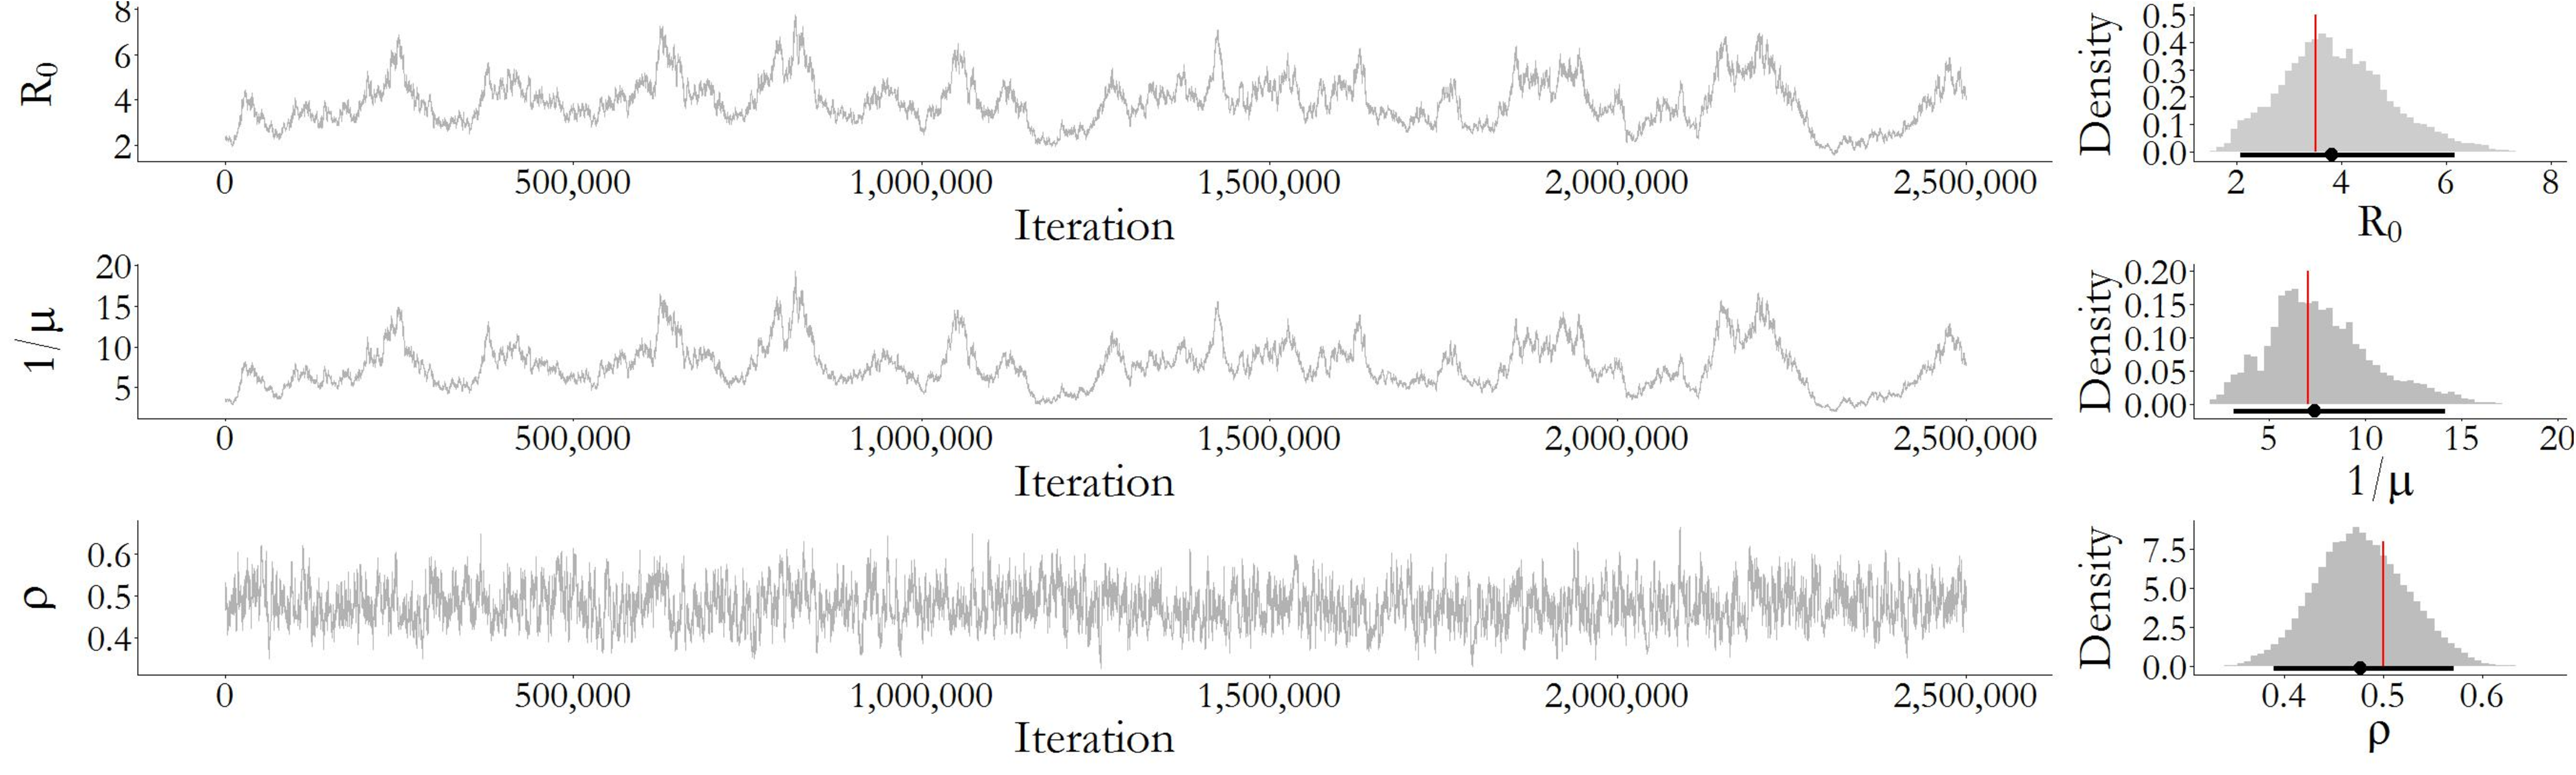
\includegraphics[width=\textwidth]{figures/lna_centered_traces}
\caption{Posterior traceplots and histograms for a single MCMC chain of an SIR model fit to Poisson distributed incidence data. MCMC targeted the posterior, \ref{eqn:lna_approximate_posterior}, alternately updating $ \bNtil|\btheta,\bY $ via elliptical slice sampling, and $ \btheta|\bNtil,\bY $ via a multivariate random walk Metropolis algorithm. $ R_0 = \beta N / \mu$ is the basic reproductive number, $ 1/\mu $ is the mean infectious period duration, and $ \rho $ is the mean case detection rate. }
\label{fig:lna_centered_traces}
\end{figure}

\subsubsection{Non--centered Parameterization}
\label{subsubsec:noncentered_parameterization}	

To alleviate 
In practice, the transition density (\ref{eqn:lna_transition_density}) could be used, as written, to approximate transition densities of the log--incidence process, $ \bNtil $ and to obtain sample paths of the incidence process, $ \bN $. However, we will make two modifications: First,  Second, for reasons that will be discussed in the next subsection, we adopt a non--centered parameterization for the log--incidence process by deterministic mapping standard normal random variables, $ \bZ\sim MVN(\bs{0},\mb{I}) $, onto LNA incidence and prevalence sample paths. The procedure for this mapping, denoted \doLNA, is presented in Algorithm (\ref{alg:doLNA}). We will denote by $ \bN(\bZ,\btheta,\mcI) $ and $ \bX(\bZ,\btheta,\mcI) $ the incidence and prevalence sample paths that are output by the \doLNA\ procedure.

\begin{algorithm}[h!]
	\caption{Mapping standard normal draws onto LNA sample paths.}
	\label{alg:doLNA}
	\begin{algorithmic}[1]
		\Procedure{doLNA}{$ \bZ,\btheta,\mcI $}
		\State \textbf{initialize: }$ \bX(t_0) \gets \bx_0,\ \bN(t_0) \gets \bs{0},\ \bNtil(t_0) \gets \bs{0},\ \bmu(t_0) \gets \bs{0},\ \bSigma(t_0) \gets \bs{0} $
		\For{$ \ell = 1,\dots,L $}
		\State $ \bmu(t_\ell),\ \bSigma(t_\ell) \gets $ solutions to (\ref{eqn:lna_ode_drift}) and (\ref{eqn:lna_ode_diffusion}) over $ (t_{\ell-1}, t_\ell] $
		\State $ \bNtil(t_\ell)\gets \bmu(t_\ell) + \bSigma(t_\ell)^{1/2}\bZ(t_\ell) $ \Comment{non--centered parameterization}
		\State $ \bN(t_\ell)\gets \bN(t_{\ell-1}) + \exp(\bNtil(t_\ell)) - \bs{1} $
		\State \textbf{restart initial conditions:} 
		\State {\hspace{0.2in} $ \bX(t_\ell) \gets \bX(t_{\ell-1}) + \bA^T(\bN(t_\ell)-\bN(t_{\ell-1})),\ \bNtil(t_\ell) \gets \bs{0},\ \bmu(t_\ell)\gets\bs{0},\ \bSigma(t_\ell)\gets\bs{0} $ }
		\EndFor
		\State \hspace{-0.25in}\Return \Comment{return incidence and/or prevalence sample paths}
		\State$\bN = \left \lbrace\bN(t_0),\bN(t_1),\dots,\bN(t_L)\right \rbrace,\ \bX = \left \lbrace \bX(t_0),\ \bX(t_1),\dots,\bX(t_\ell) \right \rbrace $
		\EndProcedure
	\end{algorithmic}
\end{algorithm}


Instead of targeting the posterior, $ \pi(\btheta,\bN|\bY) $, will target
\begin{align}
\label{eqn:lna_posterior}
\pi(\btheta,\bZ|\bY) &\propto L(\bY|\doLNA(\bZ,\btheta,\mcI))\ind{\bN(\bZ,\btheta,\mcI)\in\mcS_N^R}\ind{\bX(\bZ,\btheta,\mcI)\in\mcS_X^R}\pi(\bZ)\pi(\btheta)
\end{align}
in a DA MCMC framework as we alternate between updating $ \bZ|\btheta,\bY $ and $ \btheta|\bZ,\bY $. Note that 

\begin{itemize}
	\item LNA as deterministic mapping - i.e., define a DoLNA operation.
	\item Non--centered parameterization
	\item MCMC
\end{itemize}